% -*- mode:LaTeX; mode:flyspell; ispell-local-dictionary:"en_CA"; -*-
\documentclass{article}

% Almost always
\usepackage{enumerate}
\usepackage{booktabs}
\usepackage{amsmath, amsthm}
\usepackage{graphicx}
\usepackage[verbose,letterpaper,top=1.25in,bottom=1in,left=1.25in,right=1.25in]{geometry}

\setlength{\parindent}{0pt}
\setlength{\parskip}{\baselineskip}

% extra stuff for assignments
\newcounter{totalpoints}
\setcounter{totalpoints}{0}

\newcommand{\points}[1]{{\addtocounter{totalpoints}{#1}\textbf{[#1 points]}}}
\usepackage{environ}
\usepackage{etoolbox}
\makeatletter
\NewEnviron{answer}[1]
{\ifx\BODY\@empty
 \vspace{#1}%
\else
 {\sf \BODY}%
\fi}
\makeatother

\usepackage{totcount}
\regtotcounter{totalpoints}
\begin{document}

{\bigskip\hrule\bigskip
\huge
\noindent CMPUT 366, Winter 2022\\
Assignment \#1

\large
Due: Friday, Feb.\ 4, 2022, 11:59pm\\
Total points: \total{totalpoints}

For this assignment use the following consultation model:
\begin{enumerate}

\item you can discuss assignment questions and exchange ideas with other \emph{current} CMPUT~366 students;

\item you must list all members of the discussion in your solution;

\item you may {\bf not} share/exchange/discuss written material and/or code;

\item you must write up your solutions individually;

\item you must fully understand and be able to explain your solution in any amount of detail as requested by the instructor and/or the TAs.

\end{enumerate}

Anything that you use in your work and that is not your own creation must be properly cited by listing the original source. Failing to cite others' work is plagiarism and will be dealt with as an academic offence.

%%%%%%%%%%%%%%%%%%%%%%%%%%%%%%%%%%%%%

\bigskip\bigskip\hrule\bigskip

\vspace{1cm}
\hspace{1cm}{\bf First name:} \underline{\hspace{7cm}}

\vspace{1cm}
\hspace{1cm}{\bf Last name:} \underline{\hspace{7cm}}

\vspace{1cm}
\hspace{1cm}{\bf CCID:} \underline{\hspace{5.5cm}}\verb|@ualberta.ca|

\vspace{1cm}
\hspace{1cm}{\bf Collaborators:} \underline{\hspace{6.5cm}}

\vspace{1cm}
\bigskip\hrule\bigskip
}

\pagestyle{myheadings}
\markboth{}{CMPUT 366 --- Assignment \#1}

\clearpage
\begin{enumerate}

%------------------------------------------------------------------------------------------
\item \textbf{(Uninformed search)}
\begin{enumerate}
\item \points{15} \label{q:uninformed-graph}
Construct a graph search problem with \textbf{no more than 10 nodes} for which all of the following are true:
\begin{enumerate}[i.]
    \item Least-cost search returns an optimal solution.
    \item Depth-first search returns the highest-cost solution.
    \item Breadth-first search returns a solution whose cost is strictly less than the highest-cost solution and strictly more than the least-cost solution.
\end{enumerate}
Note that this means your search problem must have at least 3 solutions of differing costs.
Be sure to list the start and goal node(s), all edge costs and all edge directions (if your graph is directed). Draw the graph as well.

\begin{answer}{2.5in}
% Put your answer here
\end{answer}


\item \points{5}
List the \textbf{paths} in the frontier at each step of a depth first search of the problem you specified in part~(\ref{q:uninformed-graph}). Also, highlight the path that will be removed from the frontier in that step. Stop when the path removed ends in a goal state.

\begin{answer}{1in}
% put your answer here
\end{answer}

\item \points{5}
List the paths in the frontier at each step of a breadth first search of the problem you specified in part~(\ref{q:uninformed-graph}). Also, highlight the path that will be removed from the frontier in that step. Stop when the path removed ends in a goal state.

\begin{answer}{1in}
% put your answer here
\end{answer}

\item \points{5}
List the paths in the frontier at each step of a least cost search of the problem you specified in part~(\ref{q:uninformed-graph}). Also, highlight the path that will be removed from the frontier in that step. Stop when the path removed ends in a goal state.

\begin{answer}{1in}
% put your answer here
\end{answer}

\end{enumerate}

%------------------------------------------------------------------------------------------
\item \textbf{(Heuristic search)}

A farmer needs to move a hen, a fox, and a bushel of grain from the left side of the river to the right using a raft.
The farmer can take one item at a time (hen, fox, or bushel of grain) using the raft.
The hen cannot be left alone with the grain, or it will eat the grain.
The fox cannot be left alone with the hex, or it will eat the hen.
For example, the farmer cannot move from one side $x$ of the river to the other side $y$ if it would mean leaving the fox and hen together on side $x$.

The farmer can load an item onto the raft, move the raft from one side of the river to the other, or unload an item from the raft.  The farmer wants to move the items with the fewest number of trips across the river as possible, but does not care about how much time is spent loading or unloading.

\begin{enumerate}
\item \points{6} Classify this problem using the primary representational dimensions from lecture 2.

\begin{answer}{.5in}
    % put your answer here
\end{answer}

\item \points{20} \label{q:construct-rep}
Represent this problem as a graph search problem.
Be sure to include and formally describe each component of the search problem.

\begin{answer}{2.5in}
    % put your answer here
\end{answer}

\item \points{5}
What is the forward branching factor for your representation from part~(\ref{q:construct-rep})?
Justify your answer.

\begin{answer}{.75in}
    % put your answer here
\end{answer}


\item \points{10} \label{q:construct-h}
Construct a non-constant admissible heuristic for this problem.

\begin{answer}{1in}
    % put your answer here
\end{answer}


\item \points{5}
Argue that the heuristic from part~(\ref{q:construct-h}) is admissible.

\begin{answer}{1in}
    % put your answer here
\end{answer}

\item \points{60} \label{q:code}
Implement your representation from part~(\ref{q:construct-rep}) and heuristic from part~(\ref{q:construct-h}) in Python~3 by editing the \verb|River_problem| class in the provided \texttt{riverProblem.py}.
We will run your code with the command \verb|python3 riverProblem_run.py|.
Your code must complete within 2~minutes for full marks.\footnote{It should run in far less time than this.}

Submit all of your code (including provided boilerplate files) in a single zip file.

\end{enumerate}

%------------------------------------------------------------------------------------------
\item \textbf{(Local search)}

\begin{enumerate}
    \item \points{6}
    For each of the following problems, state whether graph search or local search is a more appropriate algorithm, and justify your answer.
    \begin{enumerate}[i.]
        \item Solving a Rubik's cube:
        \begin{answer}{3\baselineskip}
            %answer here
        \end{answer}
        \item Solving a maze map:
        \begin{answer}{3\baselineskip}
            %answer here
        \end{answer}
        \item Solving a Sudoku problem:
        \begin{answer}{3\baselineskip}
            %answer here
        \end{answer}
    \end{enumerate}

    \item \points{2} Is hill climbing a \textbf{complete} algorithm?  Why or why not?

    \begin{answer}{1in}
        %answer here
    \end{answer}
    
    \clearpage
    Consider the a constraint optimization problem over a single variable
    $x \in \mathcal{X} = \{0.1, 0.2, \ldots, 26.9, 27\}$, with cost graph as in the following figure:

    \begin{center}
    \begin{minipage}[c]{.5\textwidth}
    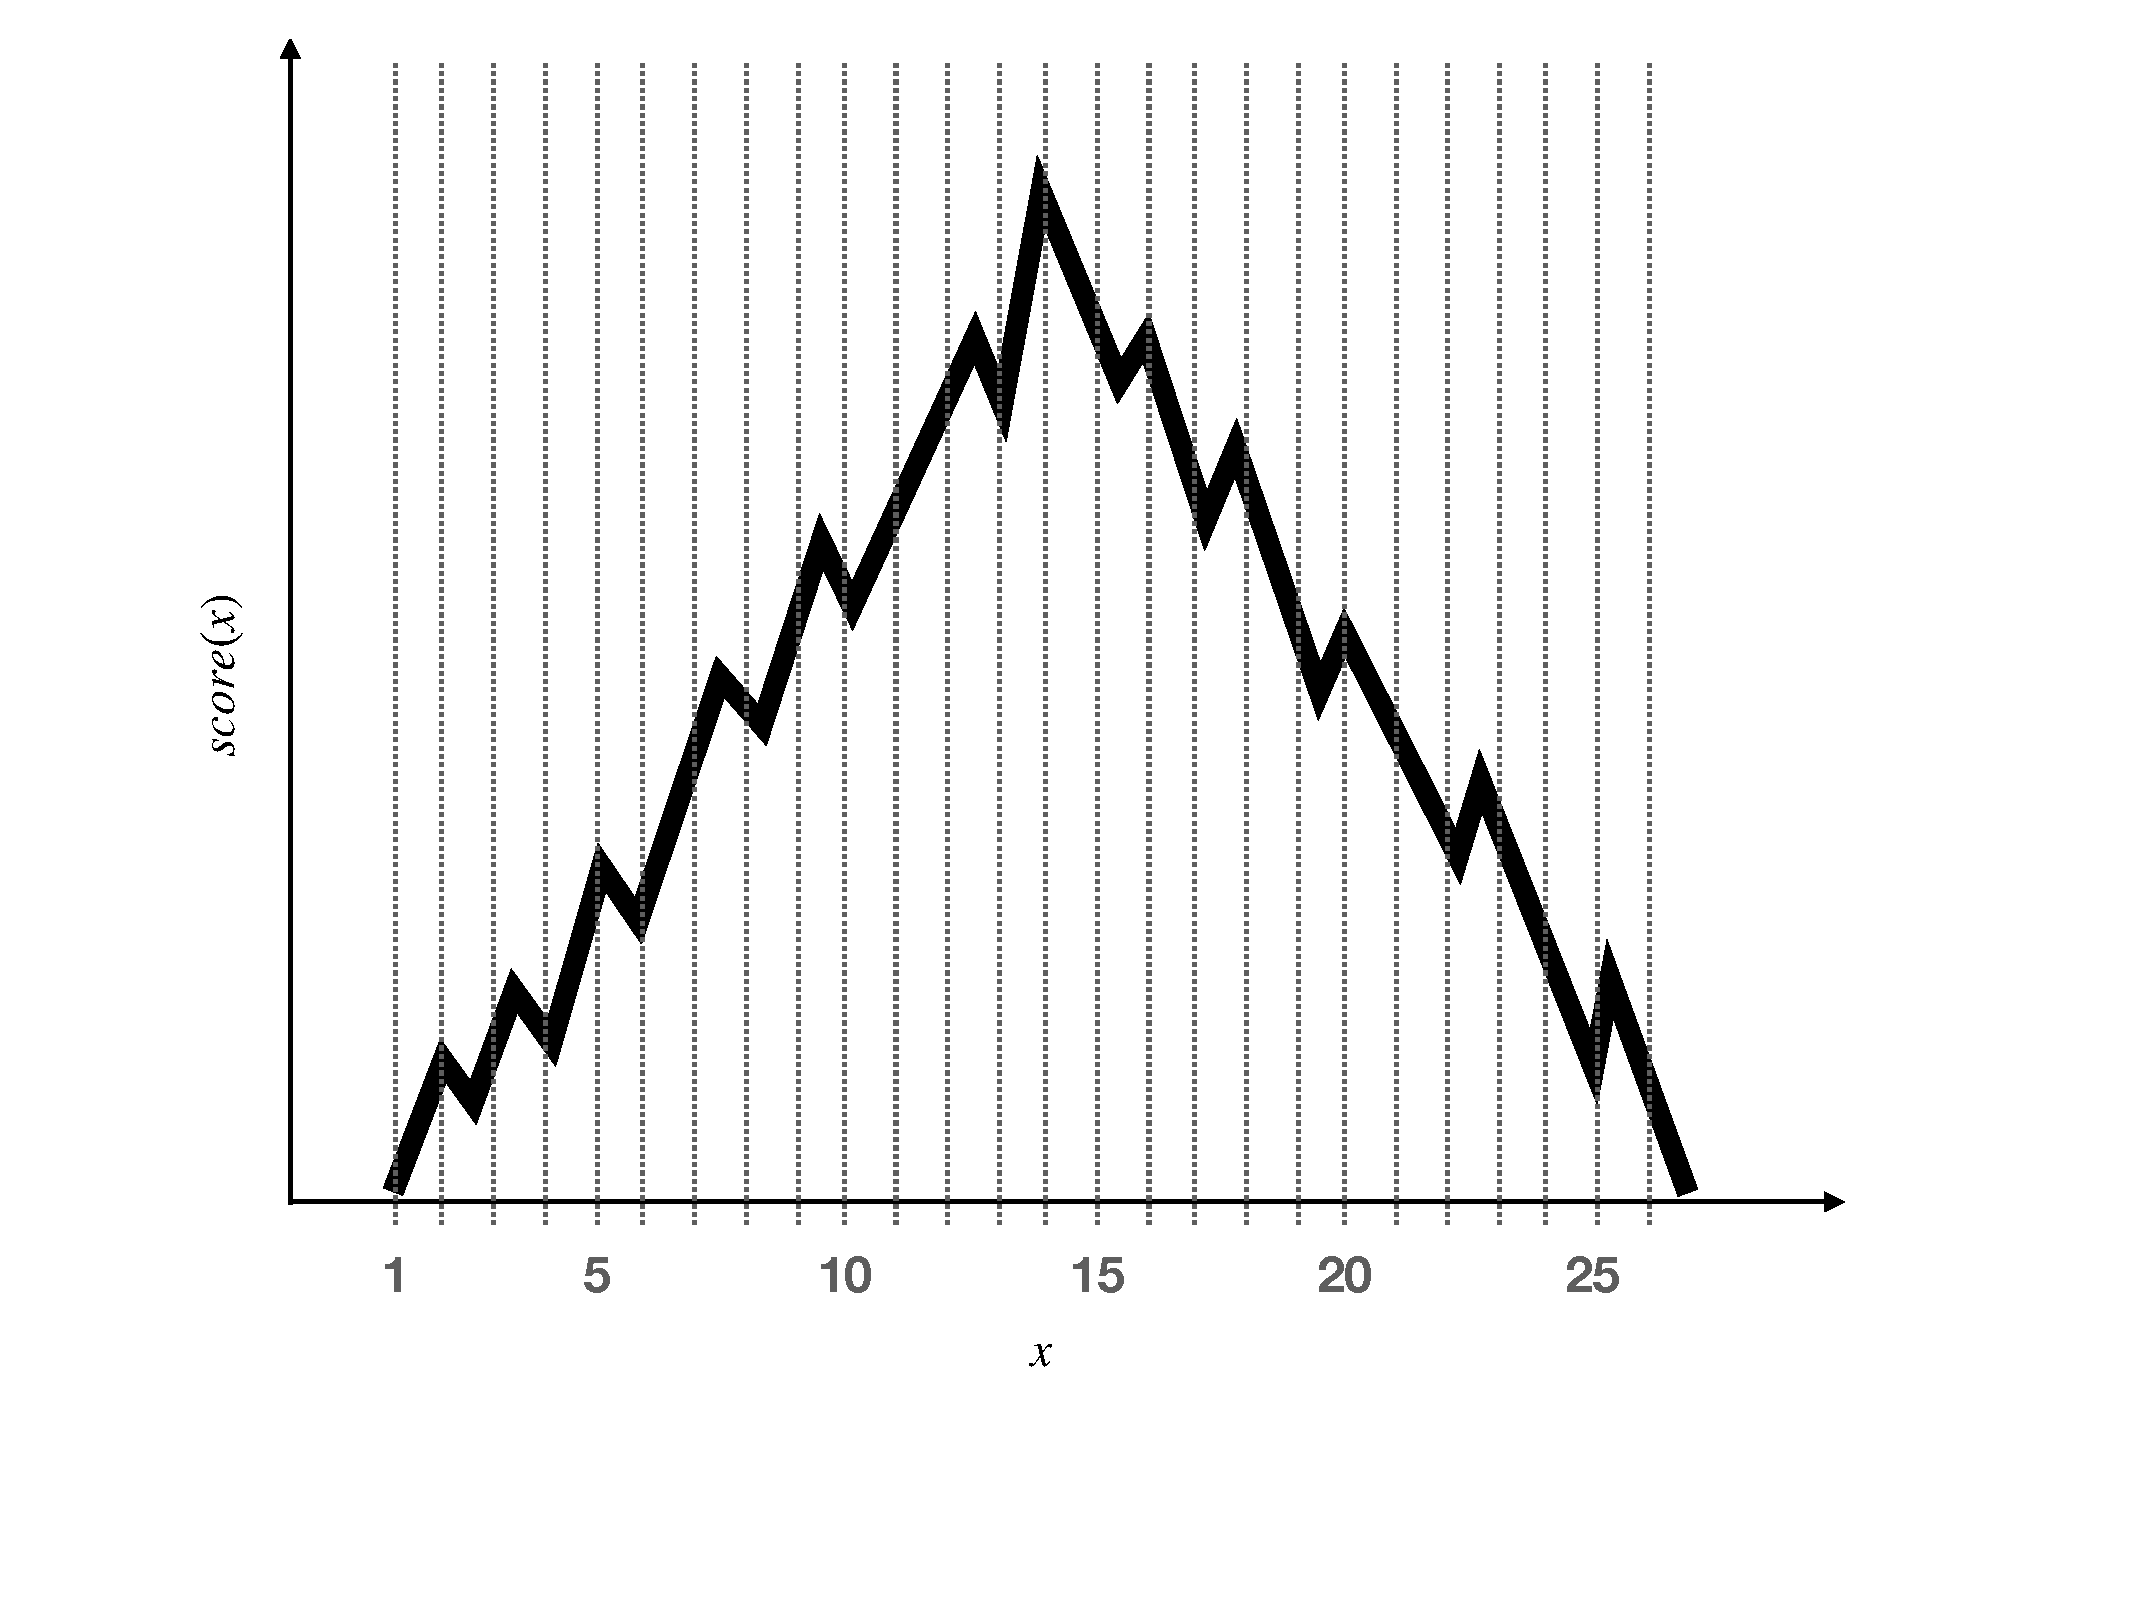
\includegraphics[width=.95\textwidth]{a1-q3.pdf}    
    \end{minipage}
    \end{center}
    
    \item \points{3} Is hill climbing on the above problem with $neighbourhood$ defined as
    \[ neighbourhood(x) = \{ y \in \mathcal{X} \mid x-0.5 \le y \le x+0.5 \} \]
    an \textbf{optimal} algorithm?  Why or why not?

    \begin{answer}{1.75in}
        %answer here
    \end{answer}

    \item \points{3} Is hill climbing on the above problem with $neighbourhood$ defined as
    \[ neighbourhood(x) = \{ y \in \mathcal{X} \mid x-2 \le y \le x+2 \} \]
    an \textbf{optimal} algorithm?  Why or why not?

    \begin{answer}{1.75in}
        %answer here
    \end{answer}
\end{enumerate}

\end{enumerate}


%------------------------------------------------------------------------------------------
\clearpage
\section*{Submission}
The assignment you downloaded from eClass is a single ZIP archive which includes this document as a PDF {\em and} its \LaTeX{} source as well as Python files needed for Question~\ref{q:code}.
%
You are to unzip the archive into an empty directory, work on the problems and then zip the directory into a new single ZIP archive for submission.

\medskip

Each assignment is to be submitted electronically via eClass by the due date.
\textbf{Your submission must be a single ZIP file containing}: 
\begin{enumerate}
    \item a single PDF file with your answers;
    \item file(s) with your Python code.
\end{enumerate}

To generate the PDF file with your answers you can do any of the following:

\begin{itemize}
    \item
    insert your answers into the provided \LaTeX{} source file between \verb|\begin{answer}| and \verb|\end{answer}|. Then run the source through \LaTeX{} to produce a PDF file;

    \item print out the provided PDF file and legibly write your answers in the blank spaces under each question. Make sure you write as legibly as possible for we cannot give you any points if we cannot read your hand-writing. Then scan the pages and include the scan in your ZIP submission to be uploaded on eClass;

    \item use your favourite text processor and type up your answers there. Make sure you number your answers in the same way as the questions are numbered in this assignment.
\end{itemize}

%\bibliography{gtdt}
%\bibliographystyle{apalike}
\end{document}

% LocalWords:  ispell
